\documentclass[12pt]{article}
\usepackage{graphicx, mathtools, natbib, amssymb, float, xspace, color, amsmath, mathrsfs}
\usepackage[margin=2.5cm]{geometry}
\usepackage{appendix}

\usepackage{tikz}
\usetikzlibrary{arrows.meta,positioning,shapes.geometric,fit,calc}


\newcommand{\Grad}{\nabla}
\newcommand{\Div}{\Grad\cdot}
\newcommand{\Curl}{\Grad\times}
\newcommand{\delsq}{\Grad^2}
\newcommand{\pd}[2]{\frac{\partial{#1}}{\partial{#2}}}
\newcommand{\ld}[2]{\frac{\text{D}{#1}}{\text{D}{#2}}}
\newcommand{\fd}[2]{\frac{\text{d}{#1}}{\text{d}{#2}}}
\newcommand{\e}{\text{e}}
\newcommand{\dirac}{\delta}
\newcommand{\identity}{\tensor{I}}
\newcommand{\pos}{\mathbf{x}}
\newcommand{\vel}{v}
\newcommand{\nvec}{\mathbf{n}}
\newcommand{\tensor}[1]{\underline{\underline{\boldsymbol{#1}}}}
\newcommand{\vect}[1]{\underline{\boldsymbol{#1}}}
\newcommand{\jump}[1]{[\![#1]\!]}
\newcommand{\pair}[1]{\boldsymbol{#1}}
\newcommand{\secondinv}{\dot{\varepsilon}_{II}}
\newcommand{\deltacmp}{\delta_\mathcal{C}}
\newcommand{\heavi}{\mathcal{H}}
\newcommand{\sr}[1]{\noindent{\textcolor{red}{\textsl{SR: #1\xspace}}}}


\title{Working Notes: Diffusion-Accommodated Grain Boundary Sliding}
\author{Zhengxuan Li}
\date{\today}

\begin{document}

\maketitle

\begin{abstract}
Add in abstract
\end{abstract}

\tableofcontents
\newpage

% ============================================================
\section{Motivation}
% ============================================================

% (to be filled)

% ============================================================
\section{Theory}
% ============================================================

\subsection{Governing equations}

The grain interiors are treated as purely elastic and isotropic, with conservation of momentum:
\begin{equation}
    \Div \tensor{\sigma} = \boldsymbol{0}, \label{eq:conservation of momentum}
\end{equation}
where $\tensor{\sigma}$ is the Cauchy stress tensor linked to the strain tensor $\tensor{\varepsilon}$ by the constitutive law.
The elastostatic equations are employed because the wavelength of elastic waves is much larger than the grain size:
\begin{equation}
    \sigma_{ij} = \lambda \varepsilon_{kk} \delta_{ij} + 2\mu \varepsilon_{ij}, \label{eq:elastic constitutive law}
\end{equation}
with the strain tensor
\begin{equation}
    \varepsilon_{ij} = \frac{1}{2}\left(\pd{u_i}{x_j} + \pd{u_j}{x_i}\right), \label{eq:strain tensor}
\end{equation}
where $\vect{u}$ is the displacement, and $\lambda$ and $\mu$ are the first and second Lam\'e parameters.

We operate in the Coble-creep (diffusion-accommodated grain-boundary sliding, DAGBS) regime \citep{raj_grain_1971, rudge_viscoelastic_2025}. Two timescales are assumed to be well-separated: tangential sliding is fast relative to the diffusion timescale, so grain boundaries slide freely; normal opening is rate-limited by grain-boundary diffusion. The grain-boundary conditions are therefore
\begin{align}
    \sigma_{ns} &= 0, \label{eq:DAGBS shear} \\
    \pd{^2 \sigma_{nn}}{\,s^2} &= -\frac{kT}{\Omega\,\delta D^{\mathrm{gb}}}\left[\pd{u_n}{t}\right], \label{eq:DAGBS normal}
\end{align}
on each grain-boundary segment $S$, where $s$ is the arc-length coordinate along $S$, $\jump{\cdot}$ denotes the jump across $S$, $k$ is Boltzmann's constant, $T$ temperature, $\Omega$ atomic volume, $\delta$ GB width, and $D^{\mathrm{gb}}$ the grain-boundary self-diffusion coefficient. Equation~\eqref{eq:DAGBS shear} states that the tangential traction is zero (free sliding). Equation~\eqref{eq:DAGBS normal} is the Raj--Ashby mass-balance law \citep{raj_grain_1971} combined with Herring's relation \citep{herring_diffusional_1950}: the surface Laplacian of the normal stress (the chemical-potential gradient driving diffusion along the boundary) is balanced by the rate of normal opening.

\subsection{Frequency-domain formulation}

For harmonic loading $\propto \e^{i\omega t}$ the time derivative becomes $\pd{}{t} \to i\omega$. Writing $t_n = \sigma_{nn}$ for the normal traction, equation~\eqref{eq:DAGBS normal} becomes
\begin{equation}
    \pd{^2 t_n}{\,s^2} = -\frac{i\omega\,kT}{\Omega\,\delta D^{\mathrm{gb}}}\jump{u_n}. \label{eq:diff-fd}
\end{equation}

\subsection{Rescaling and Maxwell time}

The natural timescale of the system is the Maxwell time
\begin{equation}
    \tau_M = \frac{\eta_{\mathrm{ss}}}{G_U}, \label{eq:maxwell time}
\end{equation}
where $\eta_{\mathrm{ss}}$ is the steady-state Coble viscosity and $G_U$ is the unrelaxed shear modulus. Both quantities are emergent properties of the homogenised microstructure and are therefore geometry-dependent. In the nondimensional model the diffusion coefficient $C_d = \Omega\,\delta D^{\mathrm{gb}} / kT$ is set equal to the per-geometry Maxwell time $\tau_M$ (measured at runtime), so that code-frequency $\omega$ corresponds to the dimensionless frequency $\tilde{\omega} = \omega\tau_M$ and the fluid--solid crossover sits near $\tilde{\omega} = 1$.

% ============================================================
\section{Discretisation}
% ============================================================

We solve the set of equations~\eqref{eq:conservation of momentum}, \eqref{eq:DAGBS shear}, and \eqref{eq:DAGBS normal} in a representative volume element (RVE) large enough to capture macroscopic viscoelastic behaviour. The RVE consists of multiple grains; displacement is discontinuous across grain boundaries. We discretise in the $H^1$ Sobolev space. Since $H^1$ basis functions are continuous across element interfaces, the RVE is partitioned into subdomains each containing a single grain.

\subsection{On each grain}

On a grain occupying domain $\Omega_i$, we test equation~\eqref{eq:conservation of momentum} against a vector test function $\vect{v} \in H^1$. Applying Green's theorem gives
\begin{equation}
    \int_{\Omega_i} \tensor{\sigma}^*(\vect{u}) : \tensor{\varepsilon}(\vect{v})\, dV
    - \int_{\partial\Omega_i} \vect{v}\cdot\tensor{\sigma}^*(\vect{u})\cdot\vect{n}_i\, dS = 0, \label{eq:ingrain weak}
\end{equation}
where $(\cdot)^*$ denotes complex conjugation.

\subsection{On grain boundaries}
\label{sec:gb}

For neighbouring grains $\Omega_i$ and $\Omega_j$ sharing interface $\Gamma_{GB} = \partial\Omega_i \cap \partial\Omega_j$, the boundary terms combine as
\begin{equation}
    \int_{\partial\Omega_i} \vect{v}\cdot\tensor{\sigma}^*\cdot\vect{n}_i\, dS
    + \int_{\partial\Omega_j} \vect{v}\cdot\tensor{\sigma}^*\cdot\vect{n}_j\, dS
    = \int_{\Gamma_{GB}} \jump{\vect{v}}\cdot\tensor{\sigma}^*\cdot\vect{n}_j\, dS,
\end{equation}
where $\vect{n}_j = -\vect{n}_i$ and $\jump{\vect{v}} = \vect{v}_i - \vect{v}_j$. Decomposing the traction $\tensor{\sigma}\cdot\vect{n}_j$ into normal and tangential components $t_n = \vect{n}\cdot\tensor{\sigma}\cdot\vect{n}$ and $t_s = \vect{s}\cdot\tensor{\sigma}\cdot\vect{n}$:
\begin{equation}
    \int_{\Gamma_{GB}} \jump{\vect{v}}\cdot\tensor{\sigma}^*\cdot\vect{n}_j\, dS
    = \int_{\Gamma_{GB}} \jump{v_s}\,t_s^* + \jump{v_n}\,t_n^*\, dS.
\end{equation}
Free tangential sliding~\eqref{eq:DAGBS shear} means $t_s \equiv 0$, so the tangential term drops entirely. We weakly enforce the normal diffusion law by solving for $t_n$ with test function $r_n$. Multiplying equation~\eqref{eq:diff-fd} by $r_n$, integrating over $\Gamma_{GB}$, and integrating by parts in $s$ gives
\begin{equation}
    \frac{i\,C_d}{\omega}\int_{\Gamma_{GB}}\pd{t_n^*}{s}\pd{r_n}{s}\, dS = \int_{\Gamma_{GB}} \jump{u_n}^* r_n\, dS,
    \label{eq:diff-weak}
\end{equation}
where $C_d = \Omega\,\delta D^{\mathrm{gb}}/kT$ and boundary terms at segment endpoints vanish after triple-junction coupling (Section~\ref{sec:junction}). The total weak form over all interior grain boundaries is
\begin{equation}
\begin{aligned}
&\sum_i \int_{\Omega_i} \tensor{\sigma}^*(\vect{u}) : \tensor{\varepsilon}(\vect{v})\, dV \\
&\quad - \int_{\Gamma_{GB}} \jump{v_n}\, t_n^*\, dS
  - \int_{\Gamma_{GB}} \jump{u_n}^* r_n\, dS
  + \frac{i\,C_d}{\omega}\int_{\Gamma_{GB}}\pd{t_n^*}{s}\pd{r_n}{s}\, dS \\
&\quad + \text{(RVE boundary terms)} = 0. \label{eq:weak-full}
\end{aligned}
\end{equation}
Note that the diffusion term contains $\partial t_n / \partial s$; the normal-traction multiplier therefore requires $H^1$ regularity \emph{along the boundary}, not merely $L^2$.

\subsection{On RVE boundaries}

For a periodic RVE, the displacement is decomposed as
\begin{equation}
    \vect{u}_{\mathrm{total}} = \vect{U} + \vect{u},
\end{equation}
where $\vect{U}$ is the macroscopic part and $\vect{u}$ the local fluctuation.
Following the micropolar model of \citet{rudge_micropolar_2021, rudge_viscoelastic_2025}, but upscaling to a Cauchy continuum and neglecting granular rotation ($\tensor{K} = \tensor{0}$), the jump across a periodic pair is
\begin{equation}
    \jump{\vect{U}} = \tensor{\Gamma}\cdot\vect{R},
\end{equation}
where $\tensor{\Gamma}$ is the (symmetric) macroscopic strain tensor and $\vect{R}$ joins the centroids of neighbouring RVEs. Unlike interior grain boundaries, the periodic faces carry \emph{both} tangential and normal multiplier blocks. The full weak form including RVE boundaries is
\begin{equation}
\begin{aligned}
&\sum_i \int_{\Omega_i} \tensor{\sigma}^*(\vect{u}) : \tensor{\varepsilon}(\vect{v})\, dV \\
&\quad - \int_{\Gamma_{GB}} \jump{v_n}\, t_n^*\, dS
  - \int_{\Gamma_{GB}} \jump{u_n}^* r_n\, dS
  + \frac{i\,C_d}{\omega}\int_{\Gamma_{GB}}\pd{t_n^*}{s}\pd{r_n}{s}\, dS \\
&\quad - \int_{\Gamma_{\mathrm{top}}\cup\Gamma_{\mathrm{right}}}
    \bigl(\jump{v_s}\,t_s^* + \jump{v_n}\,t_n^*\bigr)\, dS
  - \int_{\Gamma_{\mathrm{top}}\cup\Gamma_{\mathrm{right}}}
    \bigl(\jump{u_s}^* r_s + \jump{u_n}^* r_n\bigr)\, dS \\
&= -\int_{\Gamma_{\mathrm{top}}\cup\Gamma_{\mathrm{right}}}
    \tensor{\Gamma}^*\cdot\vect{R}\cdot\vect{n}\; r_n\, dS
  - \int_{\Gamma_{\mathrm{top}}\cup\Gamma_{\mathrm{right}}}
    \tensor{\Gamma}^*\cdot\vect{R}\cdot\vect{s}\; r_s\, dS.
\end{aligned}
\end{equation}

\subsection{Triple-junction coupling}
\label{sec:junction}

Leaving the segment-end terms in~\eqref{eq:diff-weak} as natural boundary conditions gives $\partial t_n/\partial s = 0$ at triple junctions, i.e.\ zero diffusive flux. Each grain boundary is then diffusively isolated: no mass can circulate between boundaries, yielding a standard-linear-solid response with $Q^{-1} \to 0$ as $\omega \to 0$ and no steady-state creep. To recover Coble creep we connect the per-edge $t_n$ fields at every triple junction $J$ with an exact-Lagrange coupling:
\begin{subequations}
\label{eq:junction}
\begin{align}
    &\int_{\Gamma_{ij}^{\mathrm{core}}} \xi\,\bigl(t_n^{(ij)} - \mu_J\bigr)\, dS = 0
      \quad \forall\,\xi,\quad \forall\,\text{edge }(i,j) \ni J, \label{eq:mortar} \\
    &\sum_{e \ni J} \lambda_{e,J} = 0, \label{eq:flux-balance}
\end{align}
\end{subequations}
where $\Gamma_{ij}^{\mathrm{core}}$ is a short core stub adjacent to $J$, $\mu_J$ is a reservoir potential (junction chemical potential), and $\lambda_{e,J}$ is the diffusive flux from edge $e$ into $J$. Equation~\eqref{eq:mortar} enforces stub-averaged continuity $t_n^{(e)}|_J = \mu_J$; stationarity with respect to $\mu_J$ gives the Kirchhoff flux balance~\eqref{eq:flux-balance}. This makes the per-edge fields behave as one connected network, enabling through-junction transport and hence steady-state Coble creep.

\subsection{Rigid-body-mode removal}

Pinning a corner node to the affine field injects a non-relaxing bulk stress at the pin and floors the storage modulus $C'$ at low $\omega$, masking the $C' \propto \omega^2$ divergence. We instead remove rigid-body modes with global stress-free integral constraints:
\begin{subequations}
\label{eq:rbm}
\begin{align}
    \int_\Omega u_x\, dV &= \int_\Omega (\tensor{\Gamma}\vect{x})_x\, dV, \qquad
    \int_\Omega u_y\, dV = \int_\Omega (\tensor{\Gamma}\vect{x})_y\, dV,
    & &\text{(translations)} \\
    \int_\Omega \left(\pd{u_y}{x} - \pd{u_x}{y}\right) dV
    &= (\Gamma_{yx} - \Gamma_{xy})\,|\Omega|,
    & &\text{(rotation)}
\end{align}
\end{subequations}
applied to both the real and imaginary parts of $\vect{u}$ (six Lagrange multipliers in total). The rotation target matches the rotation component of the applied affine field, which is nonzero for simple shear $\tensor{\Gamma} = \bigl(\begin{smallmatrix}0&1\\0&0\end{smallmatrix}\bigr)$. No point stress is injected, so $C'$ relaxes to its true value.

\subsection{Maxwell-time calibration}

The diffusion coefficient $C_d$ is calibrated per geometry as $C_d = \tau_M$ from two shear solves:
\begin{enumerate}
    \item \textbf{Unrelaxed modulus} $G_U$: set $C_d = 0$ (normal-locked, $\omega \to \infty$ limit) and evaluate
    $G_U = \tfrac{1}{2|\Omega|}\int_\Omega \tensor{\sigma}:\tensor{\varepsilon}\, dV$.
    \item \textbf{Steady-state viscosity} $\eta_{\mathrm{ss}}$: solve at code-$\omega = 1$ with $C_d = 1$ and evaluate
    $\eta_{\mathrm{ss}} = C''(\omega)/\omega$ on the creep plateau.
\end{enumerate}
Then $\tau_M = \eta_{\mathrm{ss}}/G_U$ and the production sweep runs with $C_d = \tau_M$, so code-$\omega$ reads $\tilde{\omega} = \omega\tau_M$. For the regular hexagonal benchmark ($\nu = 0.3$): $G_U/\mu \approx 0.82$, $\tau_M \approx 2.94 \times 10^{-5}$.

% ============================================================
\section{Problems}
% ============================================================

This section records the numerical experiments carried out to validate the
formulation and to characterise an unexpected secondary loss peak in disordered
microstructures. Throughout we write $\tilde{\omega} = \omega\tau_M$ for the
dimensionless frequency, $C'$ and $C''$ for the storage and loss parts of the
effective shear modulus, and $Q^{-1} = C''/C'$ for the attenuation.

\subsection{Hexagonal benchmark and junction-coupling convergence}
\label{sec:prob-hex}

We first validate the solver against the regular hexagonal RVE, for which the
diffusion-creep spectrum is known \citep{rudge_viscoelastic_2025}. With
$\nu = 0.3$ the per-geometry calibration of Section~\ref{sec:gb} returns
$G_U/\mu \approx 0.82$ and $\tau_M \approx 2.94\times10^{-5}$, and the swept
complex modulus reproduces the reference spectrum (Figure~\ref{fig:hex-repro}).
The intended low-frequency behaviour is recovered cleanly: with the stress-free
rigid-body-mode removal of equation~\eqref{eq:rbm} in place, the storage relaxes
as $C' \propto \omega^2$ and the loss as $C'' \propto \omega$, so that
$Q^{-1} \propto \tilde{\omega}^{-1}$ (slope $-1.000$ over more than ten decades).
With a pinned corner instead, $C'$ is floored at low $\omega$ and the divergence
is masked --- confirming that the choice of constraint, not the physics, governs
the relaxed limit.

The triple-junction coupling of Section~\ref{sec:junction} introduces a single
discretisation parameter, the length fraction \texttt{core\_frac} of the core
stub $\Gamma_{ij}^{\mathrm{core}}$ over which the mortar continuity
constraint~\eqref{eq:mortar} is enforced; smaller values approach a point-like
junction. To confirm the result does not depend on this choice we swept
$\texttt{core\_frac} \in \{0.001, 0.005, 0.01, 0.05, 0.1\}$ and compared the full
$Q^{-1}(\tilde{\omega})$ spectra (Figure~\ref{fig:corefrac}). The curves coincide
to better than $1\%$ from $\tilde{\omega} = 10^{-1}$ up to $\tilde{\omega} \sim 10^{3}$;
the only divergence ($\sim 13\%$) appears at $\tilde{\omega} \gtrsim 10^{6}$ where
$Q^{-1}$ itself is below $10^{-3}$. The junction coupling is therefore converged
and \texttt{core\_frac} is not a tuning parameter.

\begin{figure}[H]
    \centering
    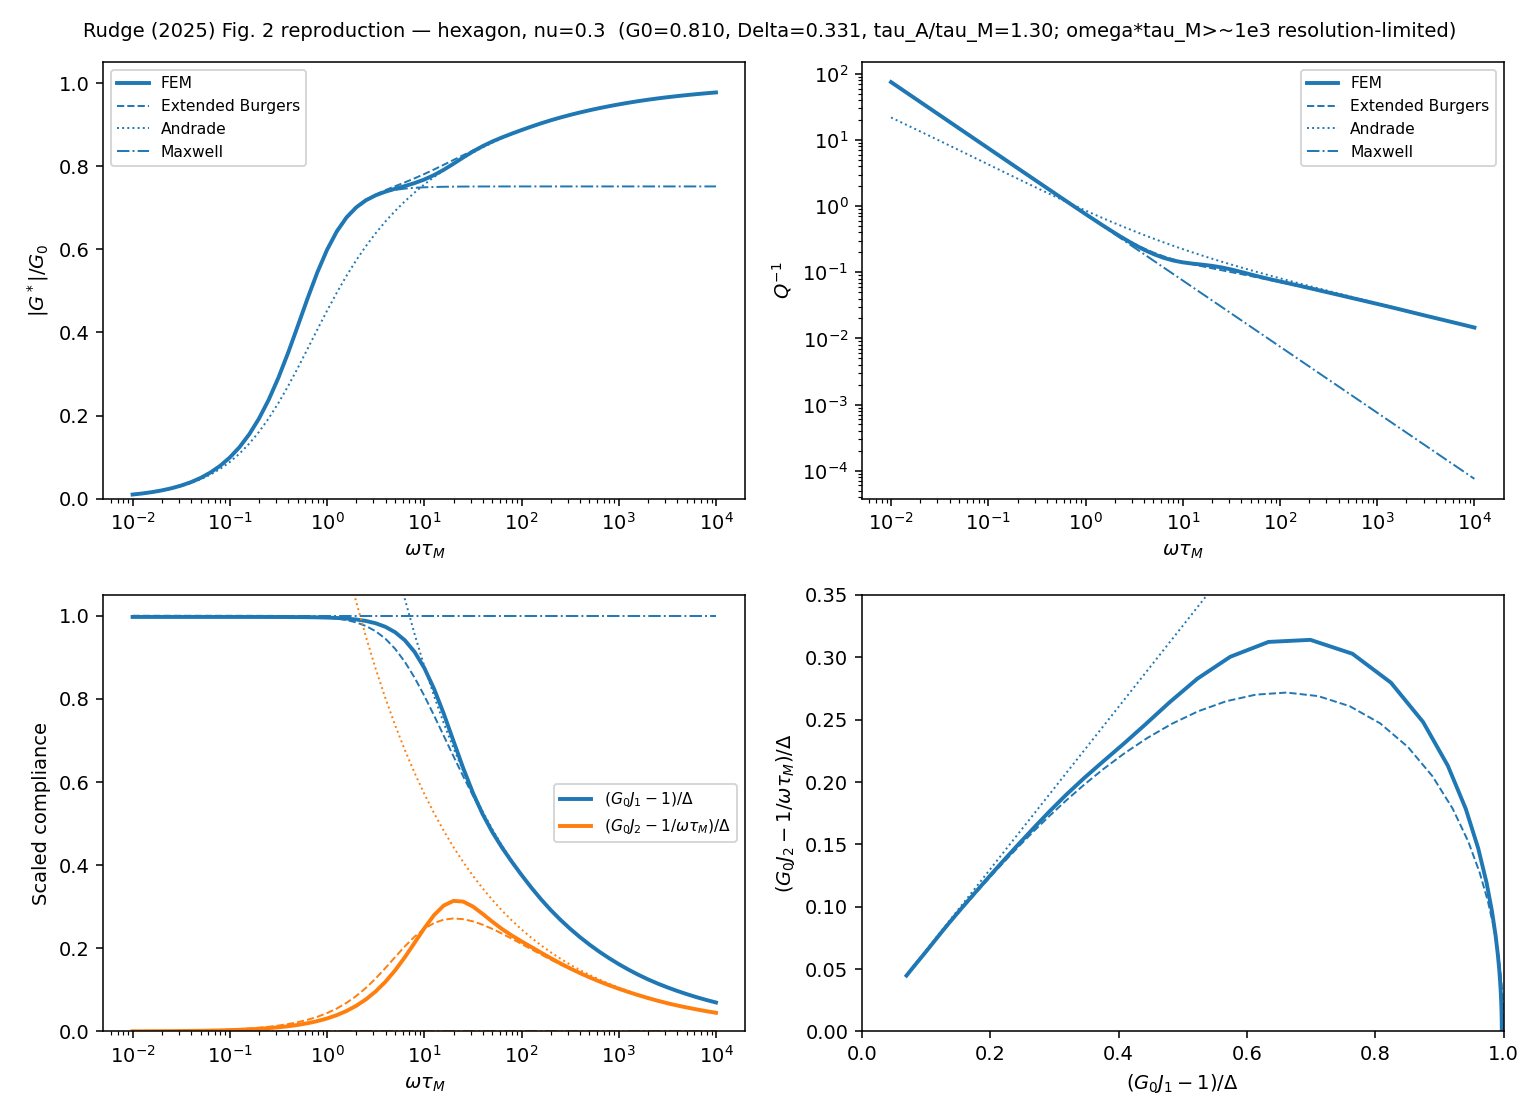
\includegraphics[width=0.9\textwidth]{figure_1_reproduction.png}
    \caption{Hexagonal benchmark ($\nu = 0.3$): swept complex shear modulus and
    attenuation against the reference diffusion-creep spectrum of
    \citet{rudge_viscoelastic_2025}. The storage modulus relaxes from the
    unrelaxed plateau $G_U$ to zero through the crossover at $\tilde{\omega} \approx 1$,
    and $Q^{-1} \propto \tilde{\omega}^{-1}$ in the creep limit.}
    \label{fig:hex-repro}
\end{figure}

\begin{figure}[H]
    \centering
    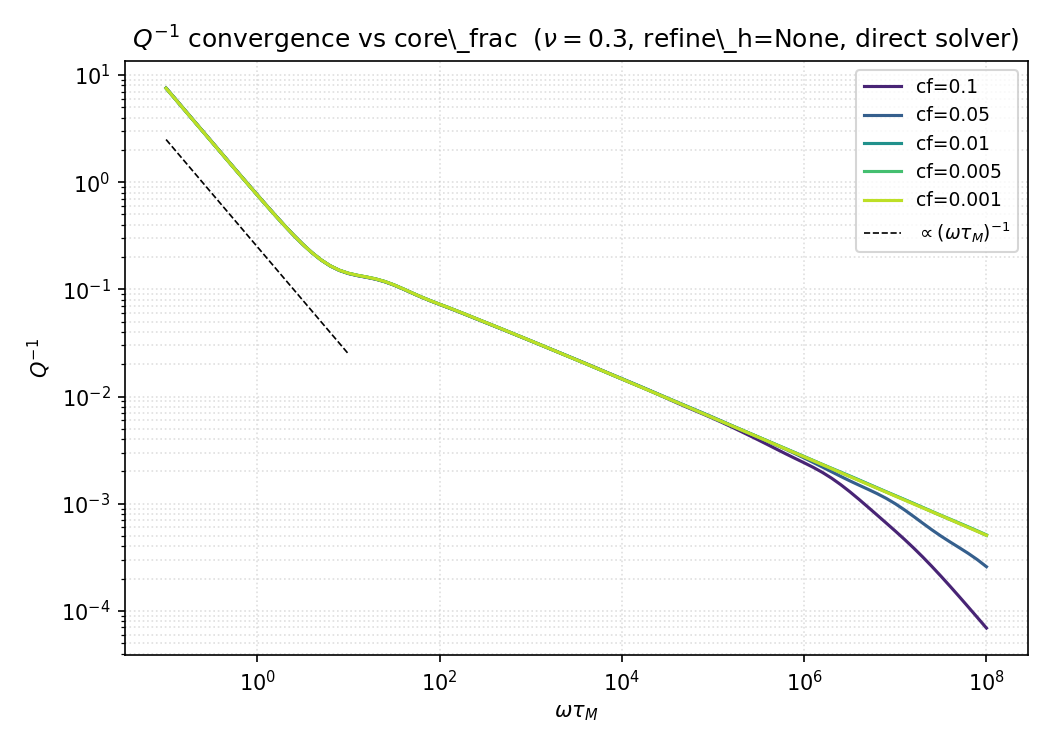
\includegraphics[width=0.62\textwidth]{figure_1_corefrac.png}
    \caption{Convergence of the attenuation spectrum $Q^{-1}(\tilde{\omega})$ with
    respect to the junction-coupling stub length \texttt{core\_frac} (hexagonal
    RVE, $\nu = 0.3$). The five curves are indistinguishable ($<1\%$) over the
    physically relevant band, demonstrating that the point-like junction limit is
    well approximated. The dashed line marks the $\tilde{\omega}^{-1}$ creep slope.}
    \label{fig:corefrac}
\end{figure}

\subsection{Random polycrystals: ensemble averaging and a secondary loss peak}
\label{sec:prob-random}

We next applied the solver to ensembles of random periodic polycrystals
(Voronoi/Neper seeds) with log-normal grain-size disorder of standard deviation
$\sigma$, sweeping $\sigma \in \{0.05, 0.10, \dots, 0.50\}$ with of order one
hundred seeds per value (about $10^3$ microstructures in total). Each seed is
calibrated and swept independently and the spectra are averaged at fixed
$\tilde{\omega}$, rescaling every seed by its own $\tau_M$
(Figure~\ref{fig:ens-overlay}).

The ensemble-mean response reproduces the hexagonal main relaxation at
$\tilde{\omega} \approx 1$, but the disordered aggregates carry an additional
feature absent from the regular hexagon: a \emph{secondary loss peak} (``bump'')
in $C''$ at high frequency, $\tilde{\omega} \gg 1$ (Figure~\ref{fig:bumps}). The
bump grows with disorder $\sigma$ and is strongly seed-dependent --- only a
minority of seeds (roughly $3\%$) show a pronounced peak. Its provenance was
initially ambiguous: because it lives at high $\tilde{\omega}$, where the shortest
grain-boundary facets are least resolved, it could plausibly be a
mesh-resolution artefact rather than a genuine relaxation. The remaining two
subsections settle this question.

\begin{figure}[H]
    \centering
    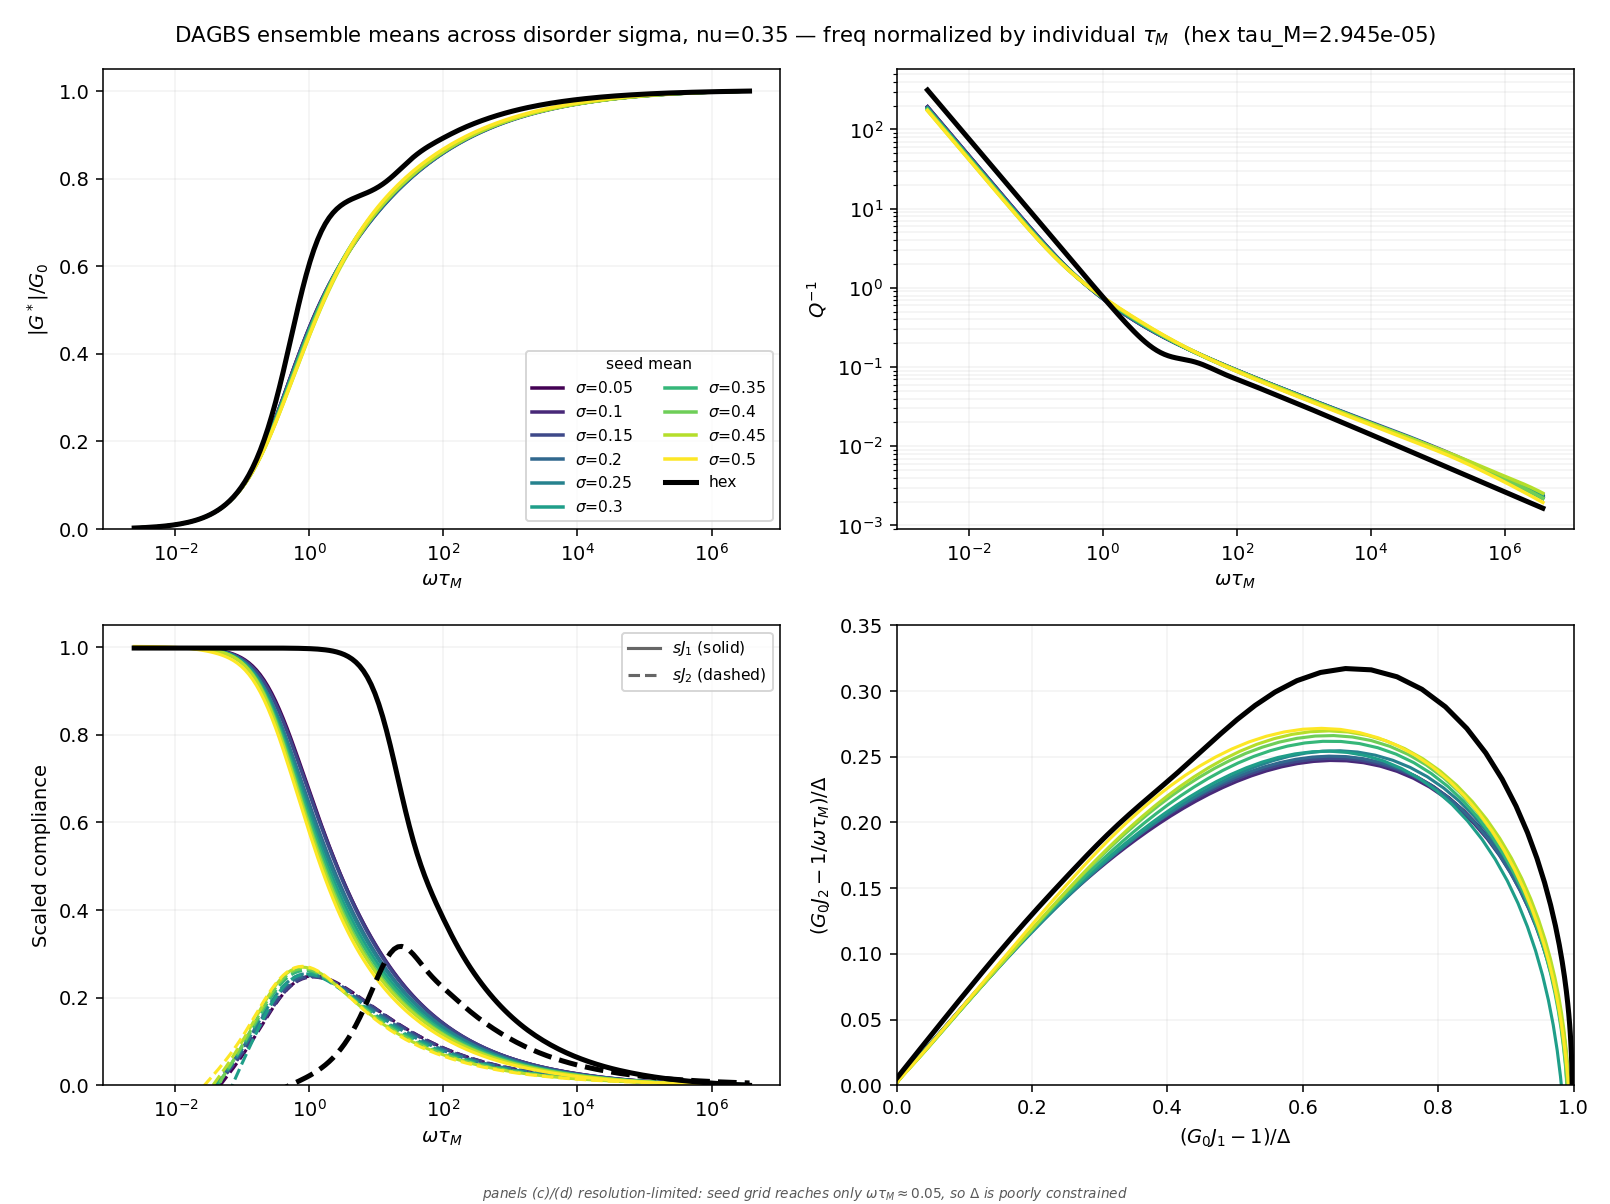
\includegraphics[width=0.95\textwidth]{figure_2_ensemble_overlay.png}
    \caption{Ensemble-mean spectra across disorder $\sigma$, each seed normalised
    by its own $\tau_M$ (black: regular-hexagon reference). Clockwise from top
    left: storage modulus, attenuation $Q^{-1}$, Cole--Cole locus, and the scaled
    storage/loss compliances. The disordered means depart from the hexagon on the
    high-$\tilde{\omega}$ (loss-compliance, dashed) side --- the signature of the
    secondary peak.}
    \label{fig:ens-overlay}
\end{figure}

\begin{figure}[H]
    \centering
    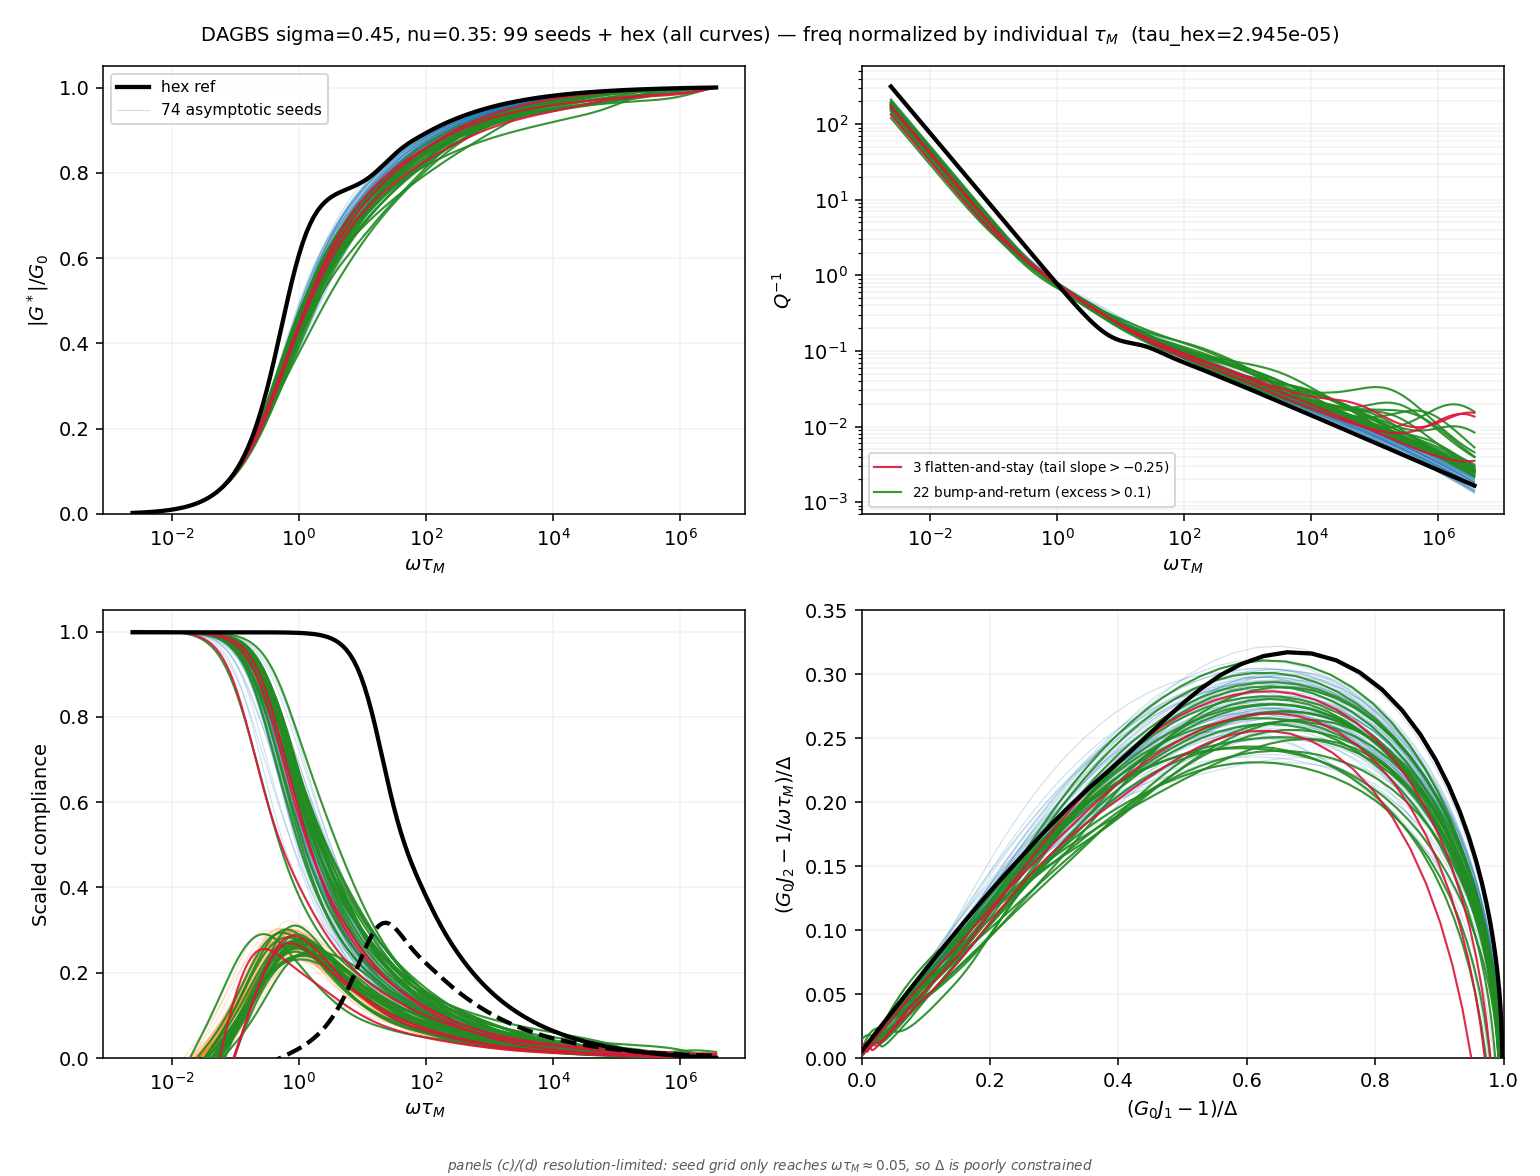
\includegraphics[width=0.95\textwidth]{figure_2_allcurves_bumps.png}
    \caption{Per-seed spectra at $\sigma = 0.45$ (individual-$\tau_M$
    normalisation). Against the hexagon reference (black) a subset of seeds
    develops a clear secondary loss peak above the main relaxation; the spread of
    its position and height across seeds is what motivated the controlled studies
    below.}
    \label{fig:bumps}
\end{figure}

\subsection{Mesh-refinement test: the secondary peak is physical}
\label{sec:prob-refine}

To decide whether the bump is a genuine relaxation or an under-resolution
artefact we refined the mesh \emph{proportionally to facet length}: interior
grain-boundary facets shorter than a cutoff are remeshed with element size
$h = L\,\texttt{refine\_frac}$, so that even sub-$h_{\max}$ slivers carry many
elements. The strongest-bump seed (seed~24, $\sigma = 0.45$) was re-swept at three
refinement levels, resolving its shortest facet from a single element up to
$\sim 165$ elements.

The criterion is decisive: a genuine relaxation set by the geometric facet length
$L$ should be \emph{insensitive} to resolution once $L$ is captured, whereas an
artefact should move or weaken under refinement. The result
(Figure~\ref{fig:refine}) is that the baseline and all refined curves are
indistinguishable, with the peak fixed at $\ln\tilde{\omega} \approx 11.6$ and
unchanged height. The bump is therefore \emph{mesh-converged and physical}. A
field decomposition of the dissipation (Figure~\ref{fig:sliver}) identifies the
mechanism: the secondary peak is a second diffusion-accommodated sliding mode
localised on the single shortest grain-boundary facet --- about $96\%$ of its
dissipation occurs on that one facet, in contrast to the collective main peak
(of order $40$ participating facets). Its relaxation frequency is set by the
facet diffusion length, $\tilde{\omega}_{\mathrm{peak}} \propto L^{-2\ldots-3}$,
which is why it does not migrate with mesh density. (We also found that one
apparent peak in the production data was instead a discontinuity introduced when
stitching the high-frequency tail onto the base sweep; re-levelling the tail at
the join removed it. This was a post-processing artefact, distinct from the
physical peaks.)

\begin{figure}[H]
    \centering
    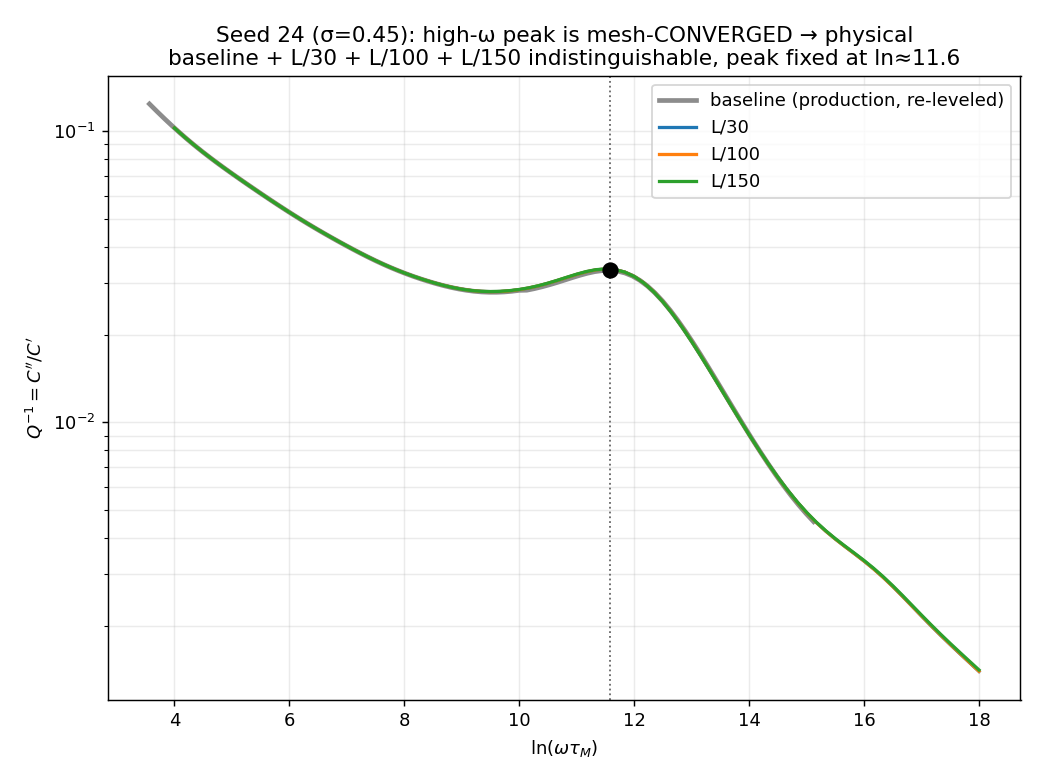
\includegraphics[width=0.8\textwidth]{figure_3_refine_convergence.png}
    \caption{Mesh-refinement convergence of the secondary peak for seed~24
    ($\sigma = 0.45$). Baseline and the three proportionally-refined meshes
    ($L/30$, $L/100$, $L/150$ element size on the shortest facet) are
    indistinguishable; the peak (marker) stays pinned at
    $\ln\tilde{\omega} \approx 11.6$. A resolution-independent peak is a genuine
    relaxation, not a discretisation artefact.}
    \label{fig:refine}
\end{figure}

\begin{figure}[H]
    \centering
    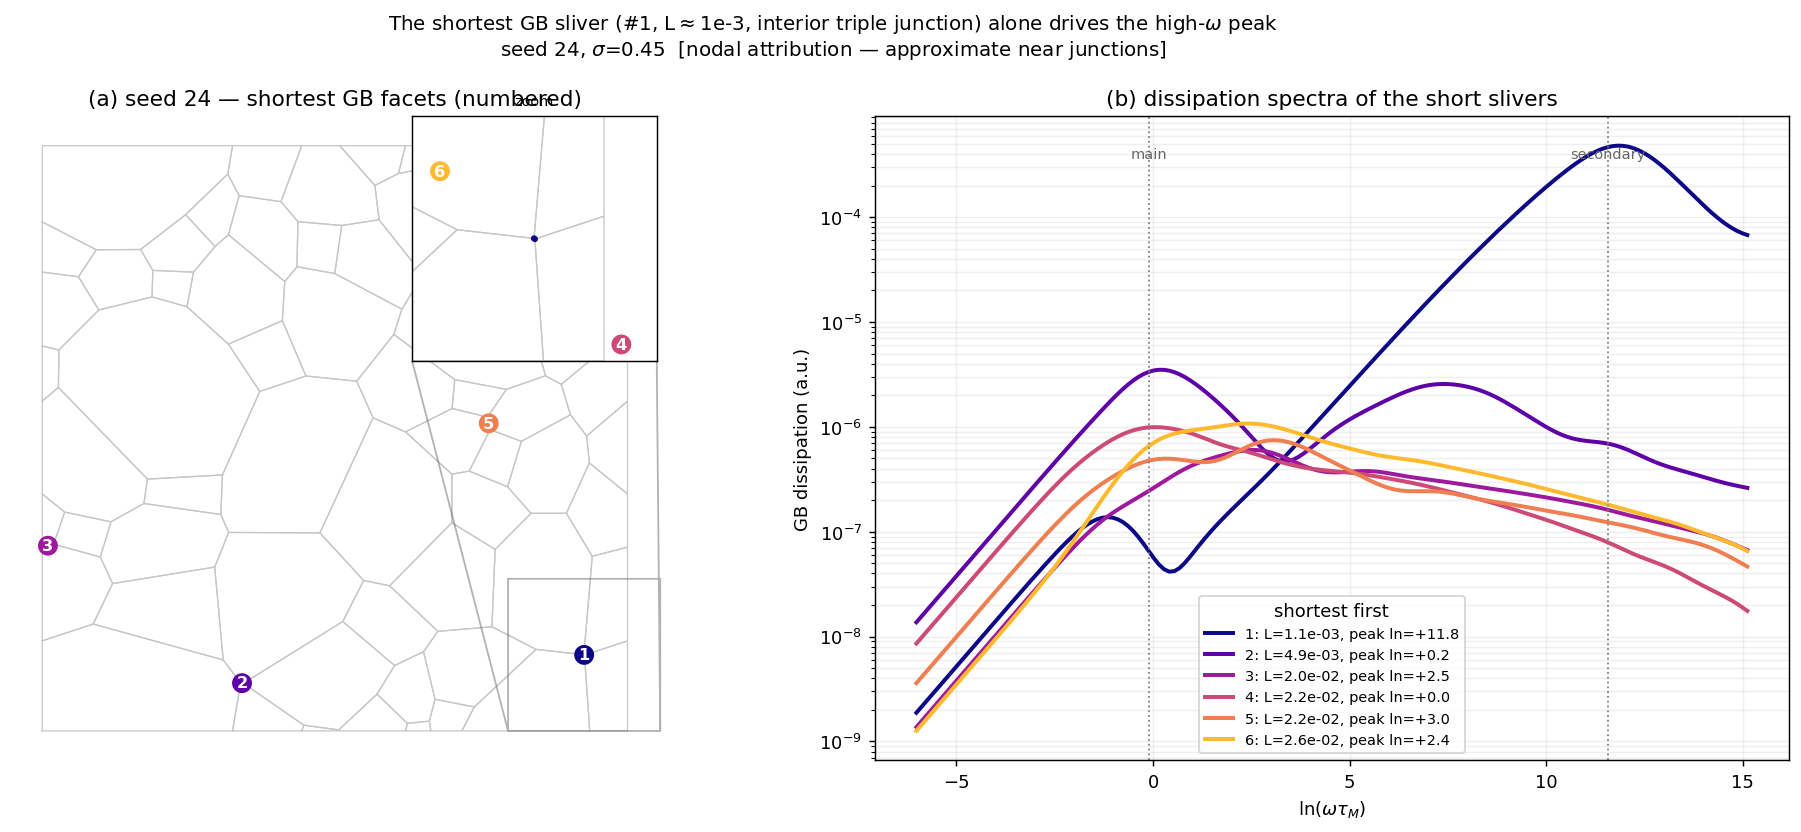
\includegraphics[width=0.8\textwidth]{figure_3_sliver_dissipation.png}
    \caption{Spatial decomposition of the secondary-peak dissipation. The loss is
    overwhelmingly concentrated on the single shortest grain-boundary facet (the
    ``sliver'' at a near-degenerate triple junction), confirming the localised,
    single-facet character of the high-frequency relaxation.}
    \label{fig:sliver}
\end{figure}

\subsection{Archimedean tilings: controlled geometry and scaling laws}
\label{sec:prob-tess}

The random ensemble establishes \emph{that} a short facet produces a secondary
relaxation but cannot cleanly isolate its scaling, because in a random seed many
quantities ($\tau_M$, neighbour topology, the facet length itself) vary together
and the shortest facets are partly resolution-limited. We therefore replaced the
random seeds with a structured Archimedean tiling carrying a single tunable small
grain: the truncated hexagonal $(3,12,12)$ (Figure~\ref{fig:geom}). A
one-parameter sweep shrinks the small triangle so that the small/large
boundary-length ratio is log-spaced down to $1/5000$, holding the domain and mean
grain area fixed.

Because the topology is hexagon-like, $\tau_M$ is set by the large grains and
stays nearly constant along the sweep; the shrinking triangles then produce
genuine secondary relaxations that march up the band as $L$ decreases. Two
distinct high-frequency modes are resolved (Figure~\ref{fig:scaling}), both
mesh-converged:
\begin{enumerate}
    \item a \emph{triangle Coble mode} with
    $\tilde{\omega}_{\mathrm{peak}} \propto L^{-3}$ (fitted slope $-3.09$ over
    $7$ points and $2.4$ decades) --- the controlled confirmation of the
    ensemble bump, whose apparent cross-seed slope ($\approx -0.70$) was
    compressed by the resolution floor on random slivers;
    \item a \emph{network ``RC'' mode} with slope $-0.99 \approx -1$, a
    collective relaxation in which the long-facet diffusion network charges
    \emph{through} the tiny triangles acting as bottleneck resistors
    ($R \propto L$ at fixed capacitance $\Rightarrow \omega \propto L^{-1}$);
    $81\%$ of its dissipation sits on the triangle facets, with a
    participation ratio of $59$ (collective).
\end{enumerate}
The $L^{-3}$ triangle mode is the same single-facet diffusion-accommodated
relaxation identified in Section~\ref{sec:prob-refine}, now with a clean exponent;
the $L^{-1}$ network mode is a distinct, collective channel that only the
controlled geometry exposes.

\begin{figure}[H]
    \centering
    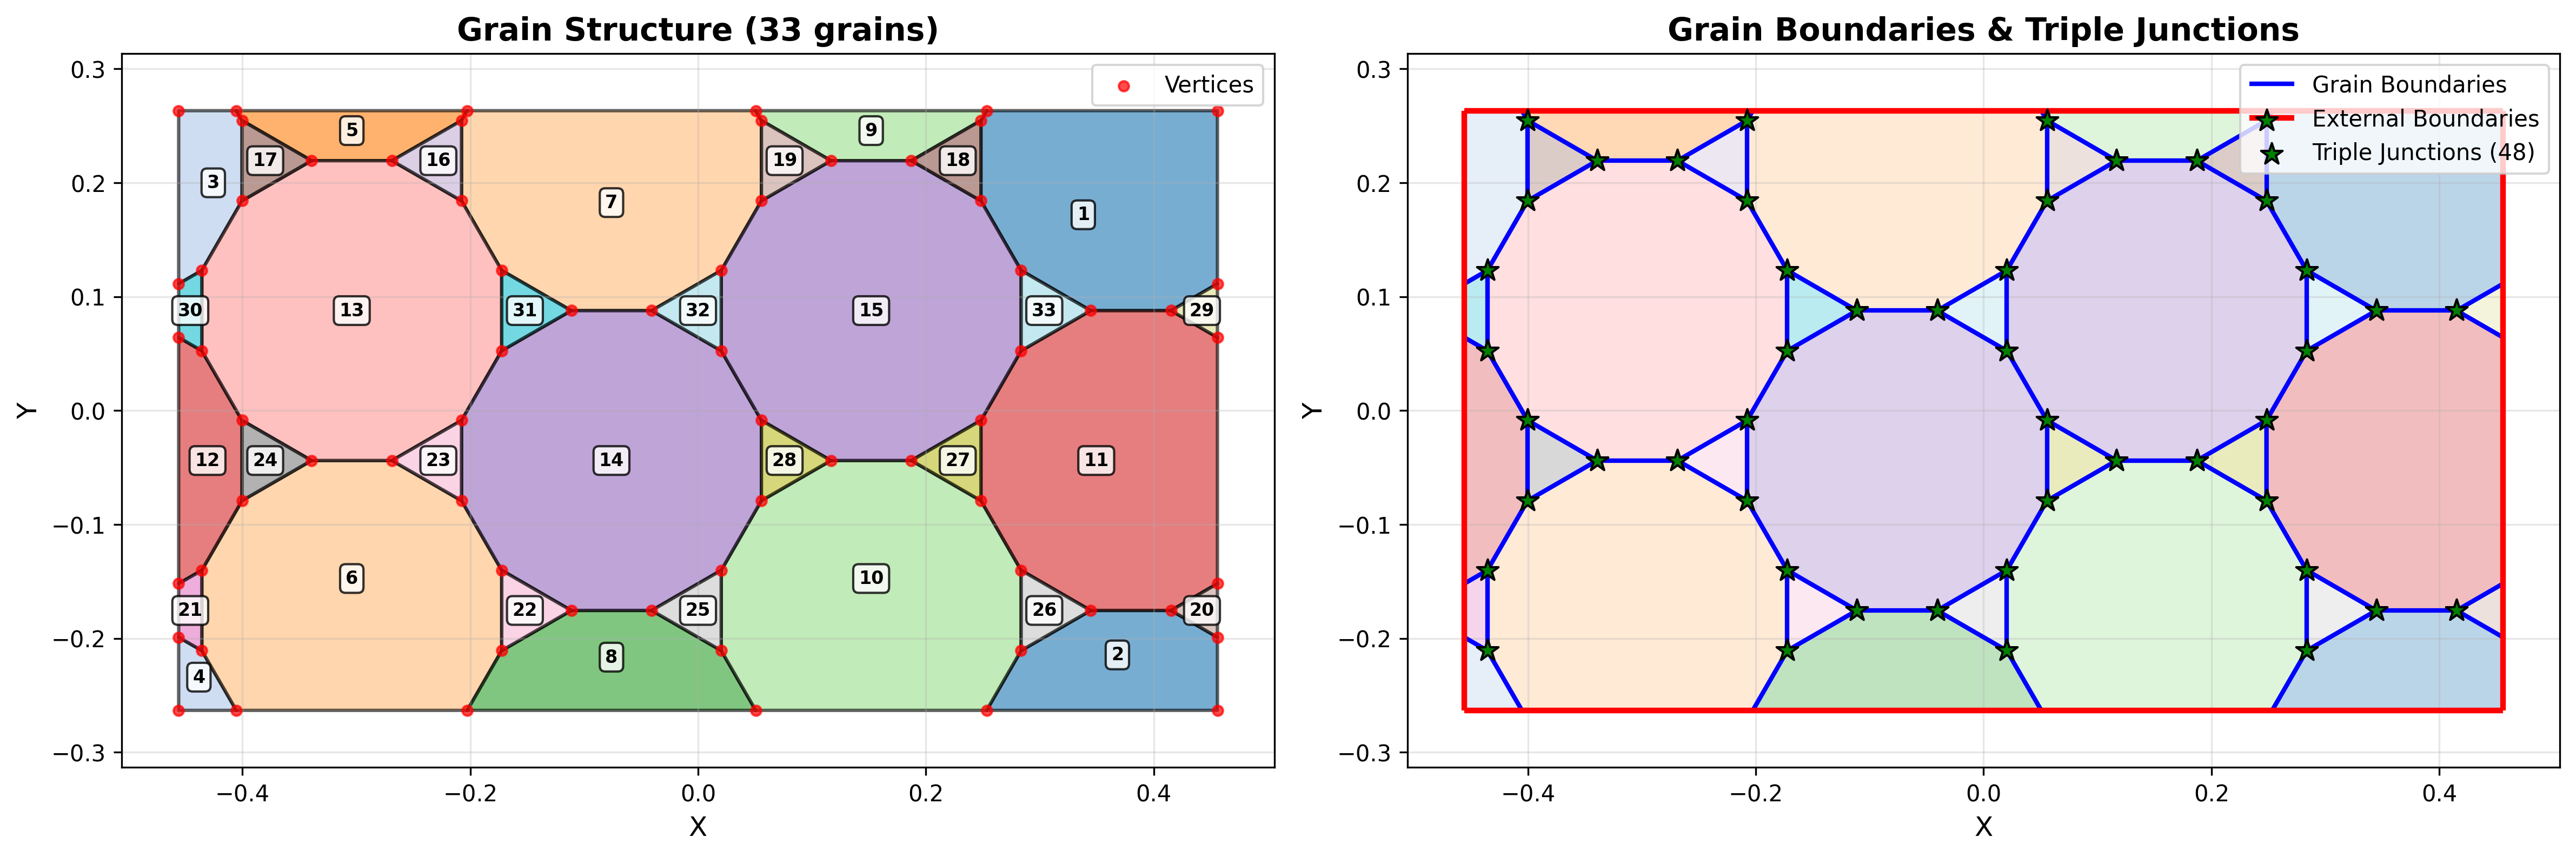
\includegraphics[width=0.55\textwidth]{figure_4_geometry_31212.png}
    \caption{Controlled Archimedean RVE: the truncated hexagonal $(3,12,12)$
    tiling --- a hexagon-like host with a single tunable shrinking triangle. It is
    the base member of a sweep that shrinks the small grain over several decades.}
    \label{fig:geom}
\end{figure}

\begin{figure}[H]
    \centering
    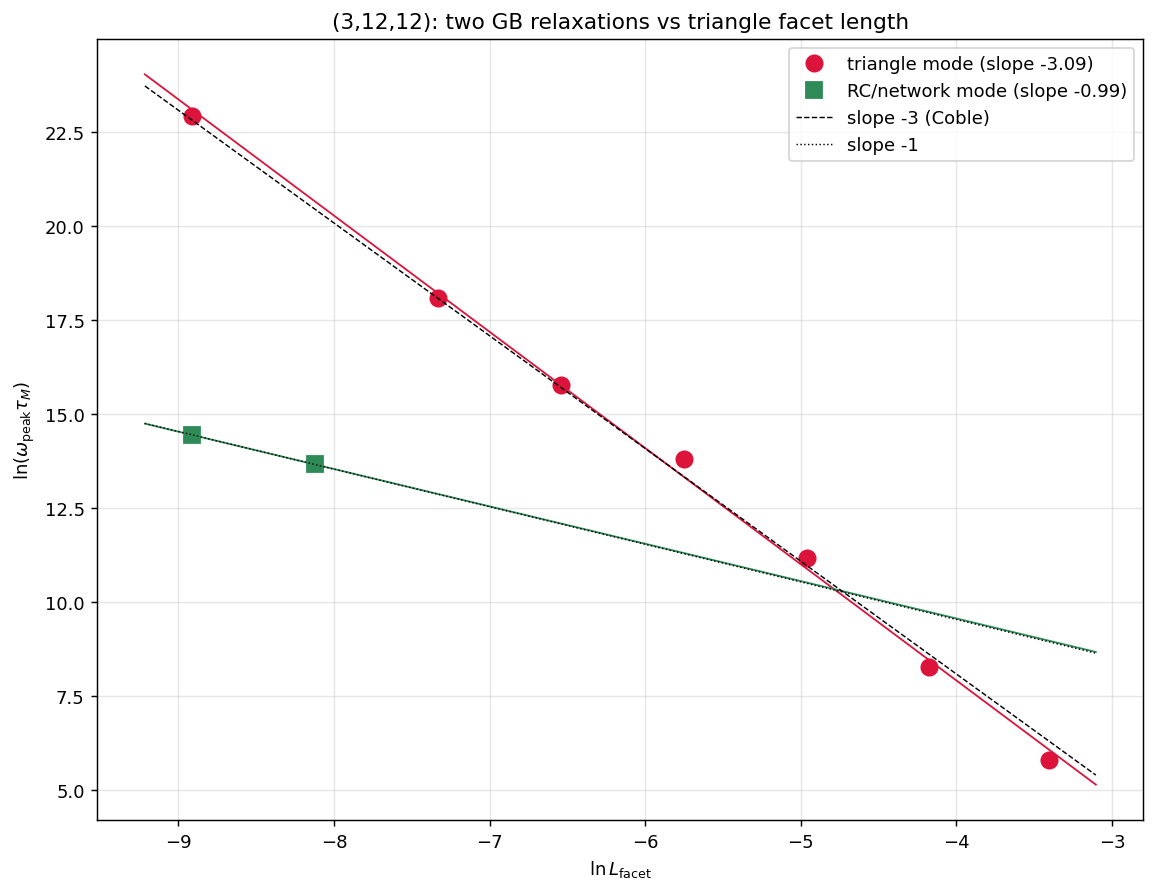
\includegraphics[width=0.8\textwidth]{figure_4_scaling.png}
    \caption{Scaling of the secondary-relaxation frequencies with triangle facet
    length $L$ for the $(3,12,12)$ family. Two power laws coexist: the triangle's
    own Coble mode (red, slope $-3.09$, i.e.\ $\omega_{\mathrm{peak}} \propto L^{-3}$)
    and the collective network ``RC'' mode (green, slope $-0.99 \approx -1$).
    Dashed/dotted lines are the ideal $-3$ and $-1$ references.}
    \label{fig:scaling}
\end{figure}

\bibliographystyle{abbrv}
\bibliography{references}

\end{document}
